\documentclass{scrartcl}
\usepackage[utf8]{inputenc} % Unicode support (Umlauts etc.)
\usepackage{hyperref} % Add a link to your document
\usepackage{graphicx} % Add pictures to your document
\usepackage{listings} % Source code formatting and highlighting
\usepackage[top=75px, bottom=75px, left=85px, right=85px]{geometry} % Change page borders
\usepackage{graphicx}
\usepackage{mathtools}


\begin{document}

\title{Computational Intelligence:
\\Report assignment 1}
\date{\today{}}

\author{
    \begin{tabular}{l r}
    	\\Tjitte de Jong - 4100794
	\\Boris Mulder - 4172930
        \\Max Spanoghe - 4331834
            \end{tabular}
  }
  
  \maketitle \thispagestyle{empty} \pagebreak
  
  \section{Questions}
  Here we will answer the questions of the first assignment.
  
  \subsection{}
  Our group will be using 10 input neurons because the objects have ten different features.
  
  \subsection{}
  The script should have 7 output neurons because there are 7 different categories for the objects.
  Hence, this is the amount of possible outcomes.
  
  \subsection{}
  For now, we have a hidden layer with 12 hidden neurons. There are many opinions about how many neurons to take, so we used the following formula: \\ \\ $\# \:hidden \:neurons = \frac{2} {3} \times (\# \:input \:neurons + \# \:output \:neurons) $
  
  \subsection{}
  We use the sigmoid function because our network should be able to deal with non-linear combinations of weights. The sigmoid function gives us a value between 0 and 1 instead of a value of a flat 0 or a flat 1, which is given by the step function.
  
  \subsection{}
  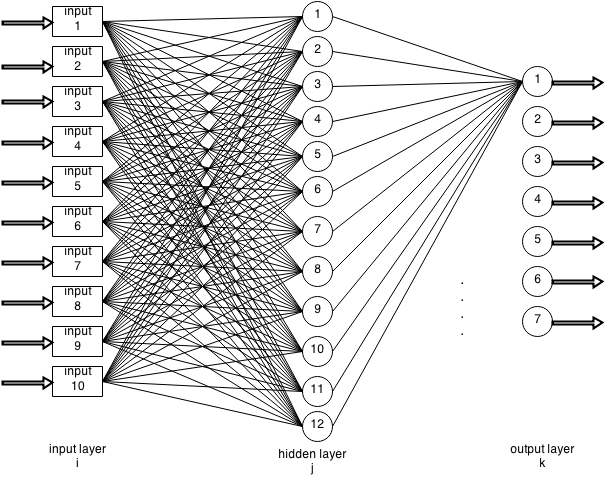
\includegraphics[scale = 0.5]{network.png}
  \\ Between the first and the second layer we have drawn all the connections, but between the second and the third we didn't just to keep a clear overview. Only the connections to the first output neuron are drawn, but of course each of output neurons is connected with each of the neurons in the hidden layer.
  
  \subsection{}
  Deviding your dataset into a training set, a validation set and a test set is very useful to overcome the problem of over fitting. You train your network with the training set to adjust the weights. Then you use the accuracy of the validation set to compare with the accuracy of the training set to determine if overfitting is occurring. When you finally have a good set weights, you use the test set to check the actual performance of the weights on this data which has not been used before.
  
  \subsection{}
  You can test the program's performance by using a test set as mentioned above. 
  
  \subsection{}
 If at any moment overfitting is occurring, you should stop training your weights on the training set. If overfitting happens, you are training your weights too hard on the training set and therefore your set of weights won't be that accurate on the test set or other sets that haven't been introduced before.
  
  \subsection{}
  With different initial weights the program could get the same result. This happens when 2 different sets of initialized weights get trained, but the hill-climbing-algorithm finds the same (local) minimum for both sets of weights. On the other hand, the different initializations of the weights
 can lead to different outcomes when the hill-climbing-algorithm finds a different (local) minimum for both sets of weights. That different (local) minimum can be lower than the other (local) minima, which means that the error is lower and thus the performance is better.
 
 \subsection{}
 For this question we tested networks with all possible amounts of hidden neurons between 7 and 30. We trained each of those 23 networks 20 times and plotted only their best result (minimal validation error and percentage of correct targets).
 See figure~\ref{fig:figure_1} and figure~\ref{fig:figure_2} on page~\pageref{fig:figure_2}.

\subsection{}
As seen on the two plots, a network with 15 hidden neurons gives a good result as the minimal validation error is the lowest of all networks we tested and the percentage of correct targets is also very good. A network with 26 neurons has a higher rate of correctness, but it also has more computational power. Therefore the network with 15 hidden neurons is actually more efficient.
See figure~\ref{fig:figure_3} on page~\pageref{fig:figure_3} for the performance of the network.


\subsection{}
The succesrate is  91.1\% on the test set. This is almost the same as on the validation set because we stop our training the moment over fitting is occurring. This way the validation set gives a good indication of what the outcome of a test set would be.

\subsection{}
The meaning and purpose of a confusion matrix is that you can see where the most errors are made. You can see which input is classified wrong according to its expected outcome. For example, you can see the times an item of type 7 is classified wrong as an item of type 1 (etc). This can be useful to locate the combinations in which lots of mistakes are made. See figure~\ref{fig:figure_4} on page~\pageref{fig:figure_4} for the confusion matrix of our final network.

\subsection{}
/

\subsection{}
/

\subsection{}
In general, the toolbox gets a better result by 1 or 2 percentages. This is because these tools use very sophisticated algorithms we don't have right now. However, sometimes it gets a totally bad result (+- 30\%) because it gets stuck in a bad local minimum. In our code this is solved by testing the network a few times with different initial weights and take the best result of those combinations. Also, the toolbox is faster with its calculation of the weights in the neural network than the solution we provided. Of course the tools are optimized in a very good way.

\pagebreak


\begin{figure}[p]
    \centering
    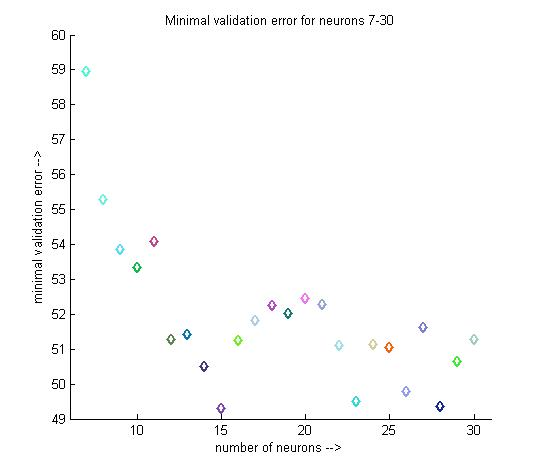
\includegraphics[width=0.8\textwidth]{Plot_Validation_Error.jpg}
    \caption{Minimal validation errors for neurons 7-30}
    \label{fig:figure_1}
\end{figure}

 \begin{figure}[p]
    \centering
    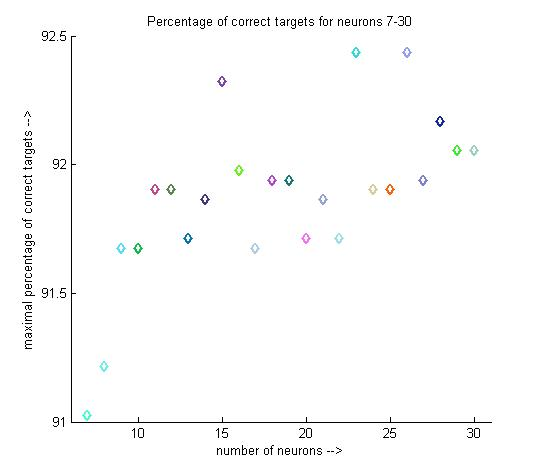
\includegraphics[width=0.8\textwidth]{Plot_Correct_Targets.jpg}
    \caption{Percentage of correct targets of neurons 7-30}
    \label{fig:figure_2}
\end{figure}

\pagebreak

\begin{figure}[p]
    \centering
    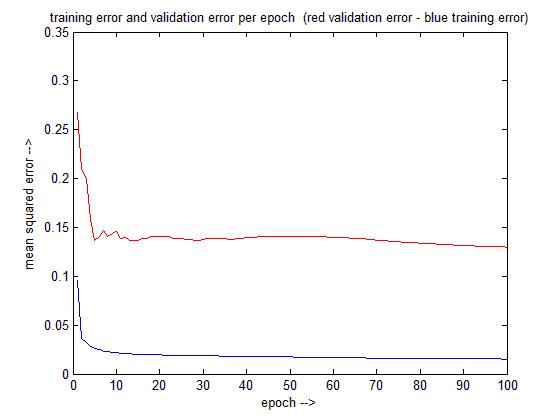
\includegraphics[width=0.8\textwidth]{validation_and_training_error.JPG}
    \caption{Validation and training error, across epochs}
    \label{fig:figure_3}
\end{figure}
\begin{figure}[p]
    \centering
    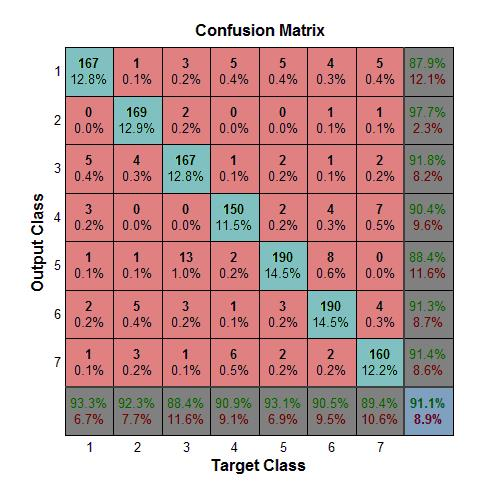
\includegraphics[width=0.8\textwidth]{Confusion_matrix.JPG}
    \caption{Confusion matrix}
    \label{fig:figure_4}
\end{figure}






 
  
\end{document}